\documentclass[../../../../main.tex]{subfiles}

\begin{document}

\section*{第1問}

\begin{proof}[解]
$(p, q)$ を直線 $2x+y=1$ 上の格子点とすると $q = 1-2p$ である。また
\[
A = \sum_{k=-10}^{10} f(k, pk+q)
\]
とおく。
\[
f(k, pk+q) = f(k, p(k-2)+1)
\]
$p \to \infty$ の時，$k \neq 2$ に対して $|p(k-2)+1| \to \infty$ となるから $f(k, p(k-2)+1) = 0$ となる。したがって
\[
\lim_{p \to \infty} A = f(2, 1)
\]
\end{proof}

\newpage

\section*{第2問}

\begin{proof}[解]
$T = \displaystyle\int_0^a P(x)P'(x)dx$, $S = \displaystyle\int_0^a \{P'(x)\}^2 dx$ とおく。
$P(x)=Ax+Bx^2$ だから，$P'(x)=A+2Bx$ で，
\[
T = \left[\frac{1}{2}\{P(x)\}^2\right]_0^a = \frac{1}{2}P(a)^2 \quad \cdots \text{①}
\]
\[
S = \int_0^a (4B^2x^2+4ABx+A^2)dx = \left[\frac{4}{3}B^2x^3+2ABx^2+A^2x\right]_0^a = \frac{4}{3}B^2a^3+2ABa^2+A^2a \quad \cdots \text{②}
\]
したがって，以下任意の $A,B\in\mathbb{R}$ に対して $T\le kS$ が成り立つ $k$ の条件を考えれば良い。①②から，
\[
T \le kS
\]
\[
\frac{1}{2}(Aa+Ba^2)^2 \le k\left(\frac{4}{3}B^2a^3+2ABa^2+A^2a\right)
\]
$a>0$ から両辺 $a$ で割って，
\[
\frac{1}{2}a(A^2+2aAB+a^2B^2) \le k\left(A^2+2aBA+\frac{4}{3}a^2B^2\right)
\]
\[
\left(\frac{1}{2}a-k\right)A^2 + (a^2B-2kaB)A + \frac{1}{2}a^3B^2 - \frac{4}{3}ka^2B^2 \le 0 \quad \cdots \bigstar
\]
これが任意の $A$ で成り立つには，$\dfrac{1}{2}a-k\le0 \iff \dfrac{1}{2}a\le k$ が必要。等号不成立の時，左辺 $f(A)$ として，$f(A)=0$ の判別式が $0$ 以下であることが必要。
\[
(a^2B-2kaB)^2 - 4\left(\frac{1}{2}a-k\right)a^2B^2\left(\frac{1}{2}a-\frac{4}{3}k\right) \le 0
\]
$a>0$ から両辺 $a^4$ で割って，
\[
\left[(a-2k)^2 - 4\left(\frac{1}{2}a-k\right)\left(\frac{1}{2}a-\frac{4}{3}k\right)\right]B^2 \le 0
\]
これが任意の $B\in\mathbb{R}$ で成立すれば良いので，$[\cdots]\le0$ ならば十分。
\[
a-2k-4\left(\frac{1}{2}a-k\right)\left(\frac{1}{2}a-\frac{4}{3}k\right) \le 0
\]
\[
(a-2k)\left[1-\left(a-\frac{8}{3}k\right)\right] \le 0 \quad \cdots \text{③}
\]
③から，$a-2k<0$ だから，
\[
1-\left(a-\frac{8}{3}k\right) \ge 0 \quad\Longrightarrow\quad k \ge \frac{3}{8}(a-1)
\]

\begin{center}
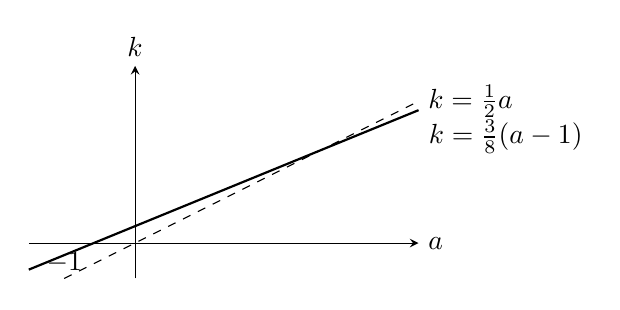
\begin{tikzpicture}[scale=0.9, >=stealth]
  \draw[->] (-1.5,0) -- (4,0) node[right] {$a$};
  \draw[->] (0,-0.5) -- (0,2.5) node[above] {$k$};
  \draw[dashed] (-1,-0.5) -- (4,2) node[right] {$k=\frac{1}{2}a$};
  \draw[thick] (-1.5,-0.375) -- (4,1.875) node[below right] {$k=\frac{3}{8}(a-1)$};
  \node[below] at (-1,0) {$-1$};
\end{tikzpicture}
\end{center}

右の図からこの時の $k$ の条件は
\[
\frac{1}{2}a < k \quad \cdots \text{④}
\]
一方，④で等号が成立する時，
\[
f(A) = a^2B^2\left(\frac{1}{2}a-\frac{4}{3}k\right) = -\frac{1}{6}a^3B^2 \le 0
\]
（$\because a>0, B\in\mathbb{R}$）だから任意の $A,B\in\mathbb{R}$ に対して★は成立する。
以上から
\[
\min k = \frac{1}{2}a
\]
\end{proof}

\newpage

\section*{第3問}

\begin{proof}[解]
$h(x) = f(x) - g(x)$ とおくと，$h(x)$ は3次以下の関数で，
\[
\begin{cases}
h(0)=h(2)=h(3) \\
h'''(x) = 6
\end{cases}
\]
②から，$h(x)$ は3次関数で（2次以下なら $h'''(x)=0$ となる），これと①及び因数定理から，$h(x)=0$ は $x=0,2,3$ を解に持ち，$h(x)=0$ は3次方程式ゆえ，高々3つの解しか持たないこととあわせて，
\[
h(x) = Ax(x-2)(x-3)
\]
と表せる。ここで $A\in\mathbb{R}\neq0$。この時，$h'''(x)=6A$ だから②に代入して $A=1$，よって
\[
h(x) = x(x-2)(x-3)
\]
ここで，$P=\displaystyle\int_1^3 f(x)dx$, $Q=\displaystyle\int_1^3 g(x)dx$ とおく。
\[
P-Q = \int_1^3 h(x)dx = \left[\frac{1}{4}x^4-\frac{5}{3}x^3+3x^2\right]_1^3 = \frac{7}{3} \quad \cdots \text{③}
\]
のもとで，
\[
F(\theta) = Pc^2+Qs^2 \quad (c=\cos\theta,\ s=\sin\theta)
\]
の $0\le\theta\le2\pi$ での $\max$ をとる $\theta$ をもとめれば良い。③から $Q=P-\dfrac{7}{3}$ だから
\[
F(\theta) = P(1-s^2)+\left(P-\frac{7}{3}\right)s^2 = -\frac{7}{3}s^2+P
\]
$0\le s^2\le1$ より，これは $\theta=0,\pi,2\pi$ で最大である。
\end{proof}

\newpage

\section*{第4問}

\begin{proof}[解]
$0<\theta<\dfrac{\pi}{2}$ 以下 $C=\cos\theta, S=\sin\theta$ と書く。

\begin{enumerate}
  \item[(1)]
  \[
  \begin{cases}
  0\le x\le C \\
  0\le y\le S
  \end{cases}
  \]
  のもとで $Q(u,v)$ ($u=x+y, v=xy$) の軌跡をもとめる。対称性からまず，$0\le\theta\le\dfrac{\pi}{4}$ でかんがえる。$u,v$ は $t$ の2次方程式 $t^2-ut+v=0$ の上記をみたす2実解である。$f(t)=t^2-ut+v$ とおく。$0<\theta\le\dfrac{\pi}{4}$ より $C\ge S$ だから，以下のいずれかである。

  \begin{center}
  \begin{tikzpicture}[scale=0.7]
    \draw[->] (-0.3,0) -- (2,0) node[right] {$t$};
    \draw[domain=-0.2:1.8, smooth] plot (\x, {(\x-0.6)*(\x-1.1)});
    \node[below] at (0.6,0) {$S$};
    \node[below] at (1.1,0) {$C$};
    \node[below left] at (0,0) {$O$};
    \node at (0.85,-1.2) {$1^\circ\ 0\le t\le S$ に2実解};
  \end{tikzpicture}
  \hspace{1cm}
  \begin{tikzpicture}[scale=0.7]
    \draw[->] (-0.3,0) -- (2,0) node[right] {$t$};
    \draw[domain=-0.2:1.8, smooth] plot (\x, {(\x-0.3)*(\x-1.4)});
    \node[below] at (0.3,0) {$O$};
    \node[below] at (0.85,0) {$S$};
    \node[below] at (1.4,0) {$C$};
    \node at (0.85,-1.2) {$2^\circ\ 0\le t\le S,\ S\le t\le C$ に1つずつ};
  \end{tikzpicture}
  \end{center}

  \textbf{$1^\circ$ の時} \quad $f(t)=0$ の判別式を $D$ とする。
  \[
  \begin{cases}
  D\ge0 \\
  f(0), f(S)\ge0 \\
  0\le \dfrac{u}{2}\le S
  \end{cases}
  \iff
  \begin{cases}
  u^2-4v\ge0 \\
  0\le u\le 2S \\
  v\ge0 \\
  S^2-uS+v\ge0
  \end{cases}
  \]

  \textbf{$2^\circ$ の時} \quad $f(0)\ge0,\ f(S)\le0,\ f(C)\ge0$
  \[
  \iff
  \begin{cases}
  v\ge0 \\
  S^2-uS+v\le0 \\
  C^2-uC+v\ge0
  \end{cases}
  \]

  $\dfrac{\pi}{4}\le\theta<\dfrac{\pi}{2}$ の時，$C$ と $S$ を入れかえれば良いから，これらを図示して下図斜線部（境界含む）。

  \begin{center}
  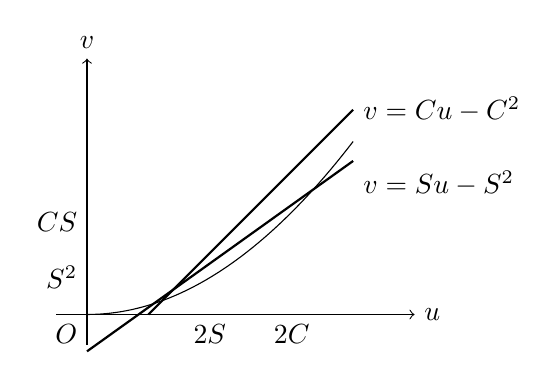
\begin{tikzpicture}[scale=1.3]
    \draw[->] (-0.3,0) -- (3.2,0) node[right] {$u$};
    \draw[->] (0,-0.3) -- (0,2.5) node[above] {$v$};
    \node[below left] at (0,0) {$O$};
    \draw[domain=0:2.6, smooth] plot (\x, {\x*\x/4});
    \draw[thick] (0.6,0) -- (2.6,2) node[right] {$v=Cu-C^2$};
    \draw[thick] (0,-0.36) -- (2.6,1.5) node[below right] {$v=Su-S^2$};
    \node[below] at (1.2,0) {$2S$};
    \node[below] at (2,0) {$2C$};
    \node[left] at (0,0.9) {$CS$};
    \node[left] at (0,0.36) {$S^2$};
  \end{tikzpicture}
  \end{center}

  この面積は，$0<\theta\le\dfrac{\pi}{4}$ の時
  \[
  S(\theta) = \int_0^{2S}\frac{1}{4}u^2du + \frac{1}{2}(C-S)(S^2+CS)-\frac{1}{2}CS^2 = \frac{2}{3}S^3+\frac{1}{2}S(C^2-S^2)-\frac{1}{2}CS^2
  \]
  $\dfrac{\pi}{4}<\theta<\dfrac{\pi}{2}$ の時，$S$ と $C$ を入れかえれば良く，$\theta=\dfrac{\pi}{4}$ の時，
  \[
  S(\theta)=\int_0^{\frac{\sqrt2}{2}}\frac{1}{4}u^2du - \frac{1}{2}\cdot\frac{\sqrt2}{2}\cdot\frac{1}{2}=\frac{\sqrt2}{24}
  \]
  で，これは $0<\theta<\dfrac{\pi}{4}$ の時の式に $\theta=\dfrac{\pi}{4}$ を代入したものにひとしい。
  \[
  S(\theta)=
  \begin{cases}
  \dfrac{1}{6}S^3+\dfrac{1}{2}SC^2-\dfrac{1}{2}CS^2 & \left(0<\theta\le\dfrac{\pi}{4}\right) \\[2mm]
  \dfrac{1}{6}C^3+\dfrac{1}{2}S^2C-\dfrac{1}{2}SC^2 & \left(\dfrac{\pi}{4}<\theta\le\dfrac{\pi}{2}\right)
  \end{cases}
  \]

  \item[(2)] $0<\theta<\dfrac{\pi}{4}$ とする。
  \[
  S\left(\frac{\pi}{2}-\theta\right) = \frac{1}{6}S^3+\frac{1}{2}CS^2-\frac{1}{2}CS^2 \cdots
  \]
  たから示された。
\end{enumerate}
\end{proof}

\newpage

\section*{第5問}

\begin{proof}[解]
\begin{enumerate}
  \item[(1)] $f(x)=e^{-x}+x-1$ とおくと，$x>0$ で $f(x)>0$ を示せば良い。
  $f'(x)=-e^{-x}+1>0$（$\because x>0$）だから，$0<x$ で $f(x)$ は単調増加で，
  \[
  f(x)>f(0)=0
  \]

  \item[(2)] $A_n = \displaystyle\prod_{k=1}^n\left(1-\frac{1}{\sqrt{k}+\sqrt{k+1}}\right)$ とおく。$1-\dfrac{1}{\sqrt{k}+\sqrt{k+1}} \ge 1-\dfrac{1}{1+\sqrt2} > 1-1 = 0$ 及び
  \[
  1-\frac{1}{\sqrt{k}+\sqrt{k+1}} = 1-\sqrt{k+1}+\sqrt{k}
  \]
  から（$A_n>0$ だから），$p_k=\sqrt{k+1}-\sqrt{k}$ とおくと
  \[
  \log A_n = \sum_{k=1}^n \log(1-p_k) \equiv B_n \quad \cdots \text{①}
  \]
  (1)から，$0<x<1$ の時，自然対数をとって
  \[
  -x > \log(1-x)
  \]
  $0<p_k<1$ だから，$x=p_k$ として
  \[
  -p_k > \log(1-p_k)
  \]
  $k$ について足して
  \[
  -\sum_{k=1}^n p_k > B_n \quad\Longrightarrow\quad 1-\sqrt{n+1} > B_n \quad \cdots \text{②}
  \]
  ①②から
  \[
  1-\sqrt{n+1} > \log A_n
  \]
  $n\to\infty$ の時，$1-\sqrt{n+1}\to-\infty$ だから，追い出しの原理より
  \[
  \log A_n \to -\infty
  \]
  $y=\log x$ は連続で，
  \[
  A_n \to +0
  \]
\end{enumerate}
\end{proof}

\newpage

\section*{第6問}

\begin{proof}[解]
$0<\alpha,\beta<1 \quad \cdots \text{①}$

\begin{enumerate}
  \item[(1)]
  \[
  p_{n+1} = \alpha p_n + (1-\beta)(1-p_n)
  \]

  \item[(2)] (1)から
  \[
  p_{n+1} = (\alpha+\beta-1)p_n + (1-\beta)
  \]
  \[
  t = \frac{1-\beta}{2-(\alpha+\beta)}
  \]
  とすると
  \[
  p_{n+1}-t = (\alpha+\beta-1)(p_n-t)
  \]
  等比数列の公式から
  \[
  p_n = (\alpha+\beta-1)^{n-1}(p_1-t)+t
  \]
  $-1<\alpha+\beta-1<1$（$\because$①）から，
  \[
  p_n \to t = \frac{1-\beta}{2-(\alpha+\beta)}
  \]
\end{enumerate}
\end{proof}

\end{document}
